\documentclass{article}
\usepackage[utf8]{inputenc}
\usepackage{graphicx}
\graphicspath{ {./images/} }

\title{RAPORT TEHNIC al proiectului SINCRON}
\author{Grigore D Valerian -  grupa 2A3}
\date{6 Decembrie 2022}

\begin{document}

\maketitle

\section{Introducere}

 Proiectul \textbf{Sincron} presupune crearea unui server TCP concurent la care se pot conecta simultan maxim N clienti. Serverul primeste mesaje, din S in S minute, de la macar M dintre clienti, unde M este strict mai mic decat N. Daca mesajele primite de la cei M clienti nu coincid, atunci serverul va trimite celor N clienti mesajul "gata", dupa care deconecteaza toti clientii. Daca mesajele coincid, serverul va trimite tuturor clientilor mesajul "continua" si va astepta urmatoarele mesaje de la alti doi clienti ai sai.


\section{Tehnologii Utilizate}

 Pentru comunicarea clienti-server vom folosi protocolul \textbf{TCP}. Un protocol, in contextul retelelor de calcuclatoare, este un set de reguli si proceduri care guverneaza modul in care datele sunt transmise. Scopul protocolului TCP este acela de a controla transferul de date in asa fel incat acesta sa fie de incredere.

\begin{itemize}
    Doua dintre caracteristicile protocolului TCP:
\end{itemize}
\begin{itemize}
    \item Toate pachetele ajung la destinatie; niciun pachet nu este pierdut.
    \item Toate pachetele sunt reasamblate in ordine.
\end{itemize}
\begin{itemize}
    Asadar, in cadrul proiectului \textbf{Sincron}, mesajele transmise de cei M clienti trebuie sa ajunga la server exact asa cum au fost trimise pentru a verifica daca acestea coincid, mai departe serverul trimitand comenzile respective ("gata" sau "continua") care trebuie sa ajunga in siguranta la cei N clienti.
\end{itemize}

\section{Arhitectura aplicatiei}

    Pe rand, clientii se vor conecta la server prin adresa IP si PORT-ul stabilite de server. Dupa conectare, clientii vor transmite date(in cazul nostru mesaje text) catre server, acesta fiind responsabil cu primirea, verificarea datelor si executarea anumitor comenzi dupa caz. Acesta are dreptul de a deconecta toti clientii comunicandu-le un anume "avertisment" inainte, sau de a-i pastra conectati.
   

\begin{figure}[t]
\begin{center}
    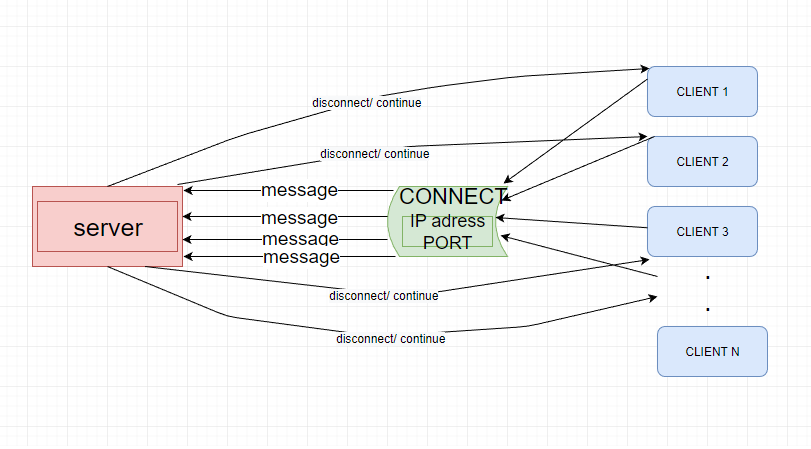
\includegraphics[width=\textwidth]{desen-bun.png}
\end{center}
\caption {Sincron Diagram}
\end{figure}


\section{Detalii de implementare}

    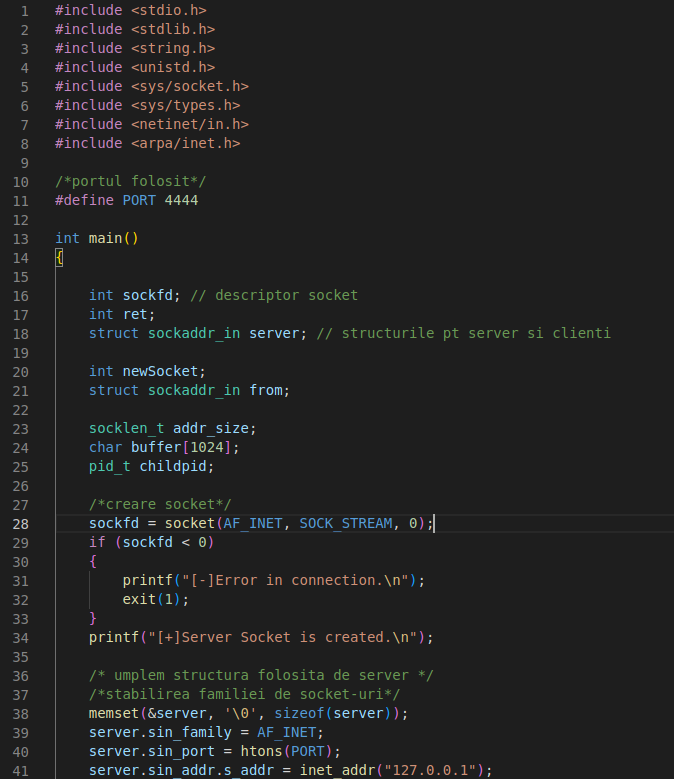
\includegraphics[width=\textwidth]{cod1.png}


    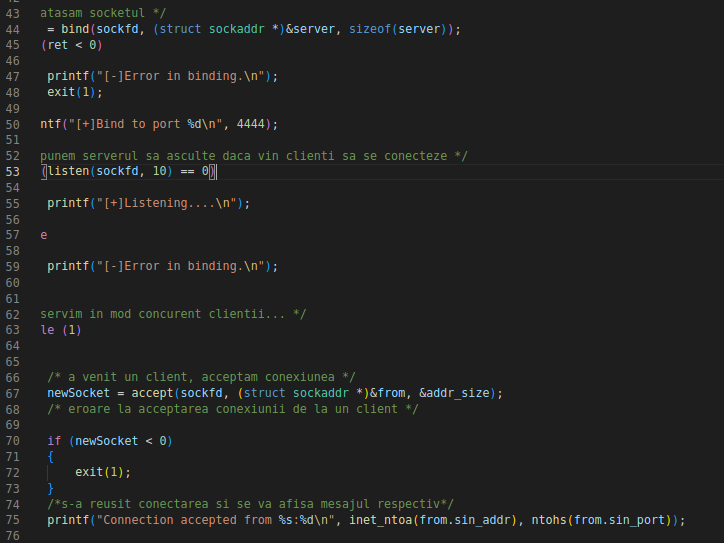
\includegraphics[width=\textwidth]{cod2.png}


  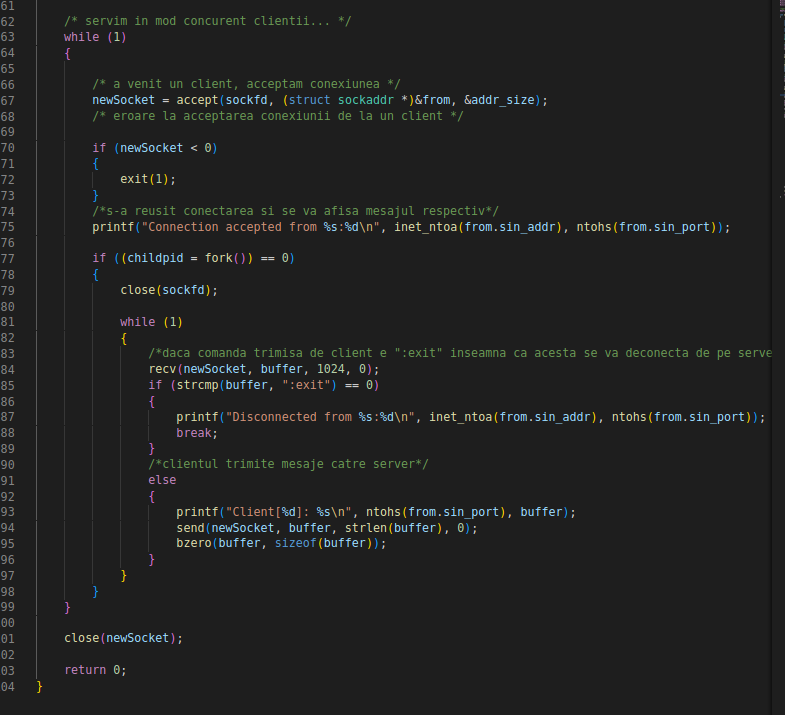
\includegraphics[width=\textwidth]{cod3.png}


\section{Concluzii}
Aplicatia nu este finalizata inca. Este nevoie de verificarea tuturor mesajelor pe care cei M clienti le trimit serverului pentru a vedea daca acestea coincid, pentru a decide daca  clientii vor fi deconectati de la server sau daca vor putea transmite in continuare mesaje. 
\section {Bibliografie}
\begin{thebibliography}{}
\begin{itemize}
\item
\url{https://profs.info.uaic.ro/~computernetworks/files/NetEx/S9/servTcpCSel.c}
\item
\url{https://profs.info.uaic.ro/~computernetworks/files/NetEx/S9/cliTcp.c}
\item
\url{https://profs.info.uaic.ro/~computernetworks/files/NetEx/S9/Makefile}
\item
\url{https://profs.info.uaic.ro/~ioana.bogdan/}
\end{itemize}
\end{thebibliography}

\end{document}

